\chapter{Curriculum Service}
\section{Abstract}
The curriculum micro-service is crucial to our design as well as the original monoliths. In the monolith, the curriculum model contained information from curriculum service and the topic service. Each of those services retrieved data from their respective repositories for the curriculum model. When converting the monolith to a micro-service architecture, the micro-services are determined by the model and the internal service communication is handled via REST templates. The services in the original monolith are now basically the internal service communication that is going on in between the business services. We chose to keep many of the same endpoints as the original monolith to reduce the necessary changes in the front end application Janus.


\section{Service Architecture}

\begin{figure}[htp]
\centering
\includegraphics[width=18cm]{images/curriculum-package}
\includegraphics[width=18cm]{images/curriculum-class}
\caption{Curriculum Service Infrastructure}
\label{fig:lion}
\end{figure}


\begin{figure}[htp]
\centering
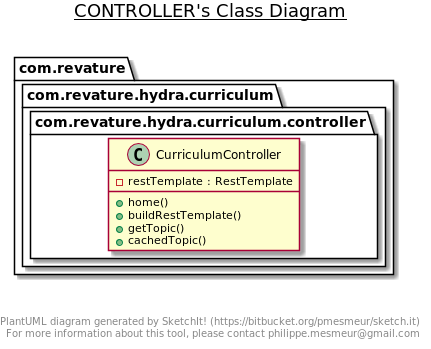
\includegraphics[width=5cm]{images/controller}
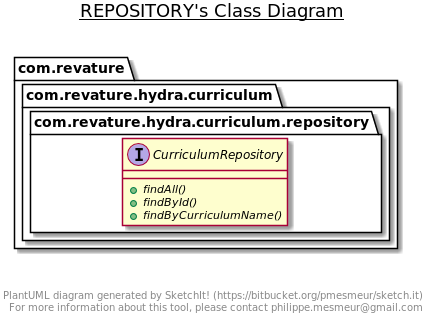
\includegraphics[width=5cm]{images/curriculumRepo}
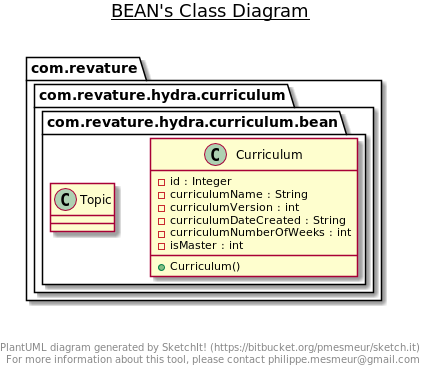
\includegraphics[width=5cm]{images/curriculumBean}
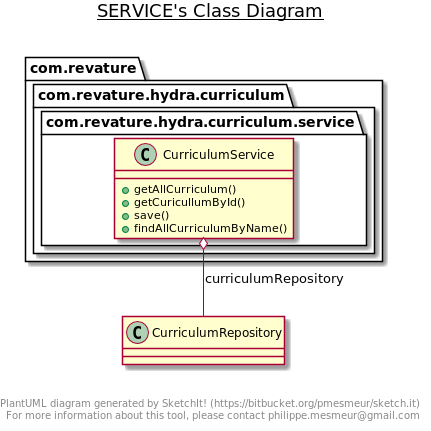
\includegraphics[width=5cm]{images/curriculumService}
\caption{Curriculum Service Hierarchy}
\label{fig:lion}
\end{figure}